\subsection{Computing the affinity graph}
\subsection{Training the neural network}

After reading the paper we realized that there was some missing informations. One of the most important points, the input and the output of the neural network, was not clear. After some research we were lucky to find the Turaga’s Phd about MALIS. Thus, we found important information we were missing.

The network predicts the affinity following each axis. As we can see on the Figure 3, in case there the network is feed by a 3D image, it output three affinity images following the axis X, Y and Z. Then we have to merge these three images in a way to obtain the complete affinity image.

\begin{figure}[!htbp]
	\centering
	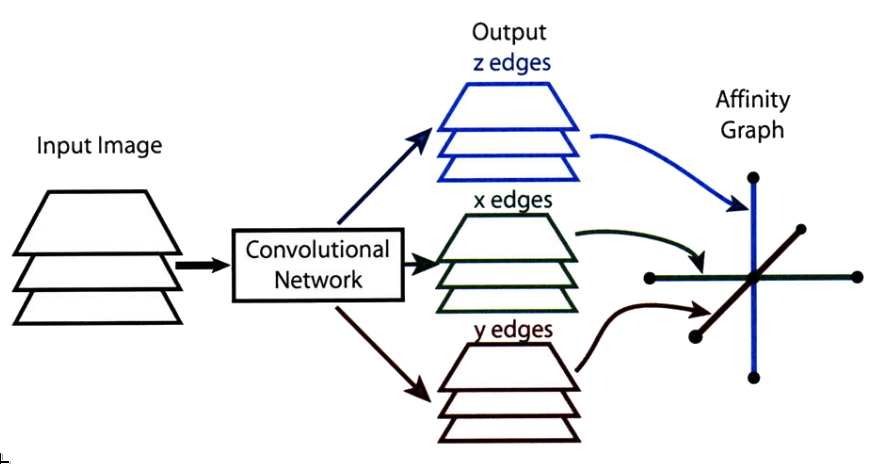
\includegraphics[width=0.8\linewidth]{./images/nn_output.png}
	\caption{Creating the affinity graph using a convolutional network. The input to the network is the 3d EM image and the desired output is a set of 3d images: one each for the x, y and z directions representing the affinity graph, from~\cite{turaga_learning_2010}}%
	\label{fig:nn_output}
\end{figure}

Another problem was to understand the input shape. In the paper, they use a patch size of 21*21*21. But it is also said that it led to an affinity classifier that use a patch with a shape of 17*17*17 to classify an affinity edge. In a first time it was kind of blur but we figured out that 17 correspond to the volume taking in account after four convolution layers, reminiscent to the proposed architecture. The patch size is also arbitrary as we are using a FCN that, by definition, don’t care about the input shape.
\newpage


As said earlier, we have to find the maximin edge in order to compute the loss. As we have to do this operation for each iteration, it is very important to guarantee a very low computational time. Our first approach was to use the Breadth First Search algorithm on the Maximum Spanning Tree efficiently created with Higra. Finally, this method was not good because our implementation was suffering from the slowness of Python. 
In our last version we are computing a Binary Partition Tree, a binary tree by altitude ordering, on the MST. This data structure is pretty pertinent as the maximin edge between to pixel i and j is the lowest common ancestor of these two pixels in the BPT. Higra also allow us to compute the loss with a larger number of pairs without an explosion of computing time because picking the lowest common ancestor is achieved in constant time.

\begin{figure}[!htbp]
	\centering
	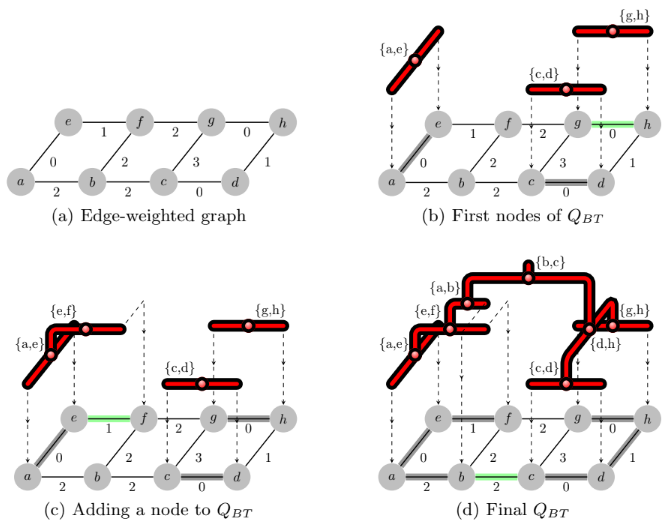
\includegraphics[width=0.7\linewidth]{./images/bpt.png}
	\caption{A simple process for obtaining a binary tree providing a strict total order relation on the edges of the MST~\cite{najman_playing_2013}}%
	\label{fig:bpt_method}
\end{figure}

We had some trouble with the interaction between Higra and Pytorch. In order to compute the loss, we have to compute a MST on the affinity image. Then we have to compute a BPT using the MST to find the maximin edge used in the loss computation. Our problem was the following: with a view to use Higra, the affinity image is turned into a graph, but by making this the gradient history is lost. Without this history it is impossible to train our NN. So, how to keep tracking the gradient history using Higra?
We found the solution in a code proposed by XXXXXXXX. Higra has a function that allow us to make the correspondence between an edge in the graph and the output affinity image. Consequently, we are able to localise the maximin edge in the output image. Due to the fact that picking an edge does not cause gradient history loss we are done.

\begin{figure}[!htbp]
	\centering
	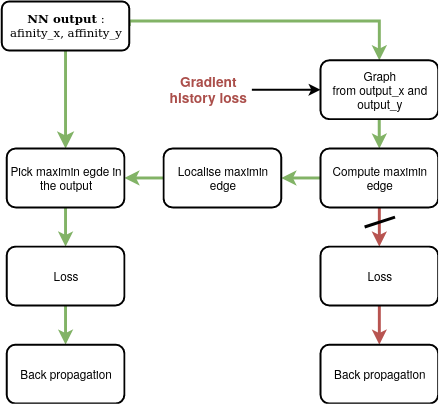
\includegraphics[width=0.6\linewidth]{./images/gradient_history.png}
	\caption{Green arrows represent out path.}
	\label{fig:bpt_method}
\end{figure}


